\documentclass{article}\usepackage[]{graphicx}\usepackage[]{color}
% maxwidth is the original width if it is less than linewidth
% otherwise use linewidth (to make sure the graphics do not exceed the margin)
\makeatletter
\def\maxwidth{ %
  \ifdim\Gin@nat@width>\linewidth
    \linewidth
  \else
    \Gin@nat@width
  \fi
}
\makeatother

\definecolor{fgcolor}{rgb}{0.345, 0.345, 0.345}
\newcommand{\hlnum}[1]{\textcolor[rgb]{0.686,0.059,0.569}{#1}}%
\newcommand{\hlstr}[1]{\textcolor[rgb]{0.192,0.494,0.8}{#1}}%
\newcommand{\hlcom}[1]{\textcolor[rgb]{0.678,0.584,0.686}{\textit{#1}}}%
\newcommand{\hlopt}[1]{\textcolor[rgb]{0,0,0}{#1}}%
\newcommand{\hlstd}[1]{\textcolor[rgb]{0.345,0.345,0.345}{#1}}%
\newcommand{\hlkwa}[1]{\textcolor[rgb]{0.161,0.373,0.58}{\textbf{#1}}}%
\newcommand{\hlkwb}[1]{\textcolor[rgb]{0.69,0.353,0.396}{#1}}%
\newcommand{\hlkwc}[1]{\textcolor[rgb]{0.333,0.667,0.333}{#1}}%
\newcommand{\hlkwd}[1]{\textcolor[rgb]{0.737,0.353,0.396}{\textbf{#1}}}%
\let\hlipl\hlkwb

\usepackage{framed}
\makeatletter
\newenvironment{kframe}{%
 \def\at@end@of@kframe{}%
 \ifinner\ifhmode%
  \def\at@end@of@kframe{\end{minipage}}%
  \begin{minipage}{\columnwidth}%
 \fi\fi%
 \def\FrameCommand##1{\hskip\@totalleftmargin \hskip-\fboxsep
 \colorbox{shadecolor}{##1}\hskip-\fboxsep
     % There is no \\@totalrightmargin, so:
     \hskip-\linewidth \hskip-\@totalleftmargin \hskip\columnwidth}%
 \MakeFramed {\advance\hsize-\width
   \@totalleftmargin\z@ \linewidth\hsize
   \@setminipage}}%
 {\par\unskip\endMakeFramed%
 \at@end@of@kframe}
\makeatother

\definecolor{shadecolor}{rgb}{.97, .97, .97}
\definecolor{messagecolor}{rgb}{0, 0, 0}
\definecolor{warningcolor}{rgb}{1, 0, 1}
\definecolor{errorcolor}{rgb}{1, 0, 0}
\newenvironment{knitrout}{}{} % an empty environment to be redefined in TeX

\usepackage{alltt}
\usepackage[hmargin = 1in]{geometry}
\usepackage{enumitem}
\usepackage{amsmath, amsthm, amssymb, amsfonts}
\setlist[2]{
font = \color{black},
before = {\color{red}}
}
\usepackage{textcomp}
\IfFileExists{upquote.sty}{\usepackage{upquote}}{}
\begin{document}





\begin{center} \LARGE
Homework 7
\end{center}
\begin{center} \Large
Due February 13, 2020 at 11:59 PM 
\end{center}



\begin{enumerate}
	\item Let $X$ be the total medical expenses incurred by a particular individual during a given year. Although $X$ is a discrete random variable, suppose its distribution is quite well approximated by a continuous distribution with pdf $f(x) = k(1 + x/2.5)^{-7}$ for $x \geq 0$.
	\begin{enumerate}
		\item {\color{black} What is the value of $k$?} (2 points)
		
		\[\int_{0}^\infty f(x) dx= 1 \Rightarrow \int_{0}^\infty k(1 + x/2.5)^{-7} dx = 2.5k (-\frac{1}{6}) (1 + \frac{x}{2.5})^{-6}\bigg|_{0}^{\infty} = \frac{k}{2.4} = 1 \]
		Therefore $k = 2.4$.
		
		
		\item {\color{black} Graph the pdf of $X$.} (2 points)
\begin{knitrout}
\definecolor{shadecolor}{rgb}{0.969, 0.969, 0.969}\color{fgcolor}

{\centering 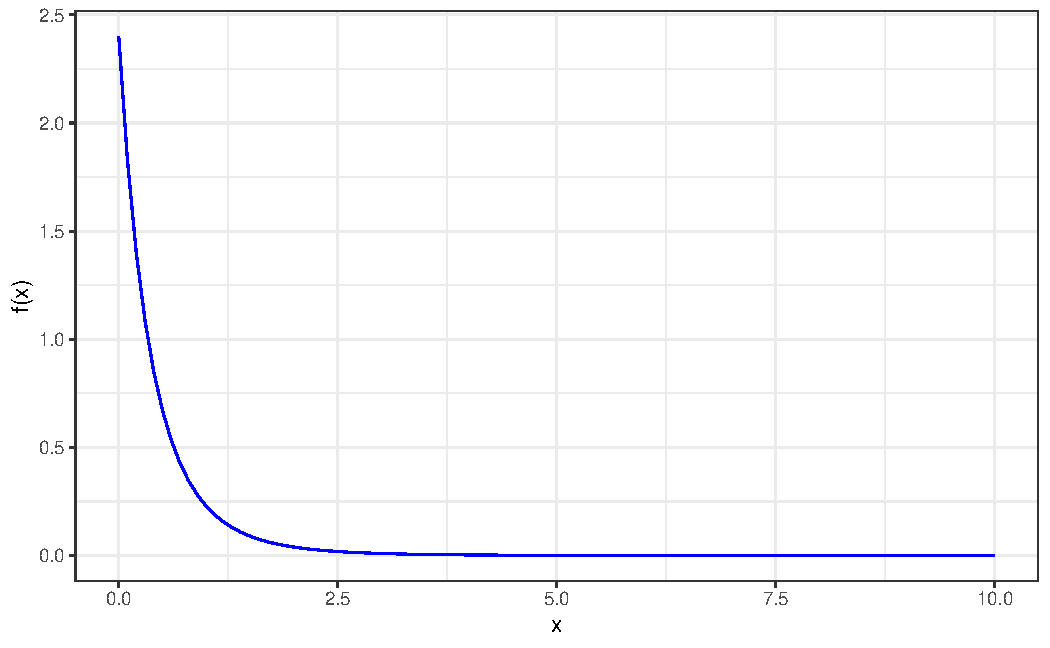
\includegraphics[width=0.6\textwidth]{figure/unnamed-chunk-2-1} 

}



\end{knitrout}
		\item {\color{black} What are the expected value and standard deviation of total mediacal expenses?} (4 points)
		
		\begin{align*}
		E(X) &= \int_{0}^\infty x \cdot 2.4 (1 + x/2.5)^{-7} dx \\
		\intertext{Let $1 + x/2.5 = u \Rightarrow x = 2.5(u-1),\, dx = 2.5du$, the limits are then 1 and $\infty$. }
		& = \int_{1}^\infty 2.5(u-1) \cdot 2.4 u^{-7} 2.5 du\\
		& = 15(-\frac{1}{5} u^{-5} + \frac{1}{6} u^{-6})\bigg|_0^\infty = 0.5
		\end{align*}
		
		\begin{align*}
		E(X^2) &= \int_{0}^\infty x^2 \cdot 2.4 x(1 + x/2.5)^{-7} dx\\
		\intertext{Let u = 1 + x/2.5,}
		& = \int_{1}^\infty (2.5(u-1))^2 \cdot 2.4 u^{-7} \cdot 2.5 du\\
		& = \frac{75}{2} \left(-\frac{1}{4} u^{-4} + \frac{2}{5} u^{-5} + u^{-7}\right)\bigg|_0^\infty = 0.625
		\end{align*}
		Therefore
		\[SD(X) = \sqrt{Var(X)} = \sqrt{E(X^2) - (E(X))^2} = \sqrt{0.625 - 0.5^2} = 0.612.\]
		
		\item 
		{\color{black} This individual is covered by an insurance plan that entails a \$500 deductible provision (so the first \$500 worth of expenses are paid by the individual). Then the plan will pay 80\% of any additional expenses exceeding \$500, and the maximum payment by the individual (including the deductible amount) is \$2500. Let $Y$ denote the amount of this individual's medical expenses paid by the insurance company. What is the expected value of $Y$? [Hint: First figure out what value of $X$ corresponds to the maximum out-of-pockect expenses of \$2500. Then write an expression for $Y$ as a function of $X$ (which involves several different pieces) and calculate the expected value of this function.] }(4 points)
		
		The maximum out-of-pocket expense occurs when $500 + 0.2 (x - 500) = 2500$. Solving this equation, we have $x = 10500$. Therefore, the amount paid by the insurance $Y$ can be wriiten as a function of $X$, $Y = g(X)$, where
		\[g(X) = \begin{cases}
		0 & , X \leq 500\\
		0.8(X - 500) & , 500 < X \leq 10500\\
		X - 2500 & , X > 10500
		\end{cases}\]
		
		Then $E(Y) = E(g(X))$, we have
		\begin{align*}
		E(g(X)) & = \int_{0}^\infty g(x) f(x) dx\\
		& = \int_{0}^{500} 0 dx + \int_{500}^{10500} 0.8(x - 500) \cdot 2.4(1 + x/2.5)^{-7} dx + \int_{10500}^\infty (x - 2500) \cdot 2.4 (1 + x/2.5)dx\\
		& = 1.22 \times 10^{-12} + 1.84 \times 10^{-18}\\
		&\approx 1.22 \times 10^{-12}
		\end{align*}
		
		
		
		{\bf Another answer:}
		If $X$ and $Y$ are in 1000s dollars as in the original question, then
		\[g(X) = \begin{cases}
		0 & , X \leq 0.5\\
		0.8(X - 0.5)& , 0.5 < X \leq 10.5\\
		X - 2.5 & , X > 10.5
		\end{cases}\]
		
		Then
		
		\begin{align*}
		E(Y ) & = E(g(X))\\
		& = \int_{0}^\infty g(x) f(x) dx\\
		& = \int_{0}^{0.5} 0 dx + \int_{0.5}^{10.5} 0.8(x - 0.5) \cdot 2.4(1 +x/2.5)^{-7} dx + \int_{10.5}^{\infty} (x - 2.5) \cdot 2.4(1 + x/2.5)^{-7} dx\\
		& = 0.1608
		\end{align*}
	\end{enumerate}

	\item 
	In a system with a large number of particles, the magnitude of velocity $X$ of these particles can be described by the Maxwell distritbuion, the pdf is given by
	\[f(x) = \begin{cases}
		 A x^2 e^{-x^2/b} & , x > 0\\
		 0 & , \mathrm{otherwise}
	\end{cases},\]
	where $b = m/(2kT)$. $k$ is the Bolzmann's constant, $T$ is the thermodynamic temperature, and $m$ is the particle mass. Suppose $b$ is known, express the constant $A$ in terms of $b$. 
	
	{\color{red} (4 points)
	
	We know the variance of the standard normal distribution is 1, so
	\[\int_{-\infty} ^{\infty} z^2 \frac{1}{\sqrt{2 \pi}}e^{-z^2/2} dz = 1 \Rightarrow \int_{-\infty}^{\infty} z^2 e^{-z^2/2} dz = \sqrt{2 \pi}.\]
	
	And with the proerty of even function, we have
	\[\int_{0}^{\infty} z^2 e^{-z^2/2} dz = \frac{1}{2} \int_{-\infty}^{\infty} z^2 e^{-z^2/2} dz = \frac{\sqrt{2 \pi}}{2}.\]
	
	Now let $x/\sqrt{b} = z/\sqrt{2} \Rightarrow x = \sqrt{\frac{b}{2}} z$.
	
	So
	\begin{align*}
	\int_{0}^\infty x^2 e^{-x^2/b} dx & = \int_{0}^\infty \frac{b}{2} z^2 e^{-z^2/2} \sqrt{\frac{b}{2}} dz\\
	& = \frac{b}{2} \sqrt{\frac{b}{2}} \frac{\sqrt{2 \pi}}{2}\\
	& = \frac{b\sqrt{b \pi}}{4}
	\end{align*}
	
	Since $\int_{0}^\infty f(x) dx = A \int_{0}^\infty x^2 e^{-x^2/b} dx = 1$, we have
	\[A \frac{b\sqrt{b \pi}}{4} = 1 \Rightarrow  A = \frac{4}{b \sqrt{b \pi}}.\]
	
	
	
	}
	
	\item P. 263: 2 (2 $\times$ 9 points)
	
	\begin{enumerate}
	\item $P(Z < -0.62) = \Phi(-0.62) = 0.2676$
	
	\item $P(Z > 1.06) = 1 - P(Z \leq 1.06) = 1 - \Phi(1.06) = 1 - 0.8554 = 0.1446$
	
	\item $P(-0.37 < Z < 0.51) = P(Z < 0.51) - P(Z \leq -0.37) = 0.6950 - 0.3557 = 0.3393$
	
	\item $P(|Z| \leq 0.47) = P(-0.47 \leq Z \leq 0.47) = P(Z \leq 0.47) - P(Z < -0.47) = 0.6808 - 0.3192 = 0.3616$
	
	\item $P(|Z| > 0.93) = P(Z < -.93) + P(Z > 0.93) = 2 P(Z < -0.93) = 2 (0.1762) = 0.3524$
	
	\item $P(-3 < Z < 3) = P(Z < 3) - P(Z \leq -3) = 0.9987 - 0.0013 = 0.9974$
	
	\item Looking up 0.90 in the body of the table, $\# \approx 1.28$
	
	\item $P(|Z| < \#) = 0.90$ is equivalent to $P(Z < \#) = 0.95$ by symmetry. So $\# \approx 1.645$.
	
	\item $P(|Z| > \#) = 0.03$ is equivalent to $P(Z < \#) = 1 - 0.03/2 = 0.985$ by symmetry. So $\# \approx 2.17$ 
	
	\end{enumerate}
	\item P. 263: 3 (2 $\times$ 8 points)

	{\color{red} Probabilities involving $X$ are just areas under the normal curve with $\mu = 43.0$ and $\sigma = 3.6$. Each of these areas has an equal corresponding area under the standard normal curve. Define $Z = \frac{X - 43.0}{3.6}$. Then $Z$ is a standard normal random variable. Re-express each of the problems below in terms of $Z$.  }
		\begin{enumerate}
	\item $P(X < 45.2) = P(Z < 0.61) = 0.7291$
	
	\item $P(X \leq 41.7) = P(Z \leq -0.36) = 0.3594$
	
	\item $P(43.8 < X < 47.0) = P(0.22 < Z < 1.11) = P(Z < 1.11) - P(Z \leq 0.22) = 0.8665 - 0.5871 = 0.2794$
	
	\item $P(|X - 43.0| \leq 2.0) = P(-0.56 \leq Z \leq 0.56) = P(Z \leq 0.56) - P(Z < -0.56) = 0.7123 - 0.2877 = 0.4246$
	
	\item $P(|X - 43.0| > 1.7) = 1 - P(|Z| \leq 0.47) = 1 - (P(Z \leq 0.47) - P(Z < -0.47)) = 1 - (0.6808 - 0.3192) = 0.6384$
	
	\item $P(X < \#) = 0.95$ is equivalent to $P(Z < \frac{\# - 43.0}{3.6}) = 0.95$. So 
	\[\frac{\# - 43.0}{3.6} \approx 1.645 \Rightarrow \# \approx 48.922\]
	
	\item $P(X \geq \#) = 0.3$ is equivalent to $P(X < \#) = 0.7$, which is equivalent to $P(Z < \frac{\# - 43.0}{3.6}) = 0.70$. So
	\[\frac{\# - 43.0}{3.6} \approx 0.52 \Rightarrow \# \approx 44.872\]
	
	\item $P(|X - 43.0| > \#) = 0.5$ is equivalent to $P(|\frac{X - 43.0}{3.6}| \leq \frac{\#}{3.6}) = 0.95$. This is equivalent to $P(|Z| \leq \#/3.6) = 0.95 \Rightarrow P(Z \leq \#/3.6) = 0.975$. So
	\[\frac{\#}{3.6} = 1.96 \Rightarrow \# = 7.056.\]
  
	\end{enumerate}
\end{enumerate}
%\newpage 
%\nocite{*}
%\bibliographystyle{plainnat} 
%\bibliography{}
\end{document}

